%-B--------------------------------------------------------------------------B-%
\begin{frame}[allowframebreaks]
\frametitle{Définitions}

\begin{block}{Corpus}

Un \textbf{corpus} est un ensemble de documents (textes, images, vidéos, etc.) 
regroupés dans une optique précise.\\[0.5em]

Dans le cadre de ce cours~: \alert{\fbox{corpus $\to$ corpus de textes}}\\[0.5em]

Plusieurs caractéristiques sont à prendre en compte pour la création d'un corpus
bien formé~:

	\begin{itemize}
		\item la taille;
		\item le langage;
		\item le temps couvert par les textes du corpus;
		\item le registre de langage.
	\end{itemize}

\end{block}

Source~: \url{http://fr.wikipedia.org/wiki/Corpus}

\framebreak

\begin{block}{Taille}

Le corpus doit évidemment atteindre une taille critique pour permettre des 
traitements statistiques fiables.

    \begin{itemize}
        \item Si un corpus est utilisé pour construire des modèles de langue, 
              quelle doit être sa taille minimum~? 1M mots, 10M mots, etc.
    \end{itemize}

\end{block}

\begin{block}{Langage}

Un corpus \textbf{monolingue} bien formé doit nécessairement couvrir une seule 
langue, et une seule déclinaison de cette langue (e.g.~français de France et 
français du Québec).

\end{block}

\framebreak

\begin{block}{Période couverte}

Le temps joue un rôle important dans l'évolution du langage~: le français parlé 
aujourd'hui ne ressemble pas au français parlé il y a 200 ans ni, de façon plus 
subtile, au français parlé il y a 10 ans, à cause notamment des néologismes.

\end{block}


\begin{block}{Registre de langage}

Un corpus construit à partir de textes scientifiques ne peut être utilisé pour 
extraire des informations sur les textes vulgarisés, et un corpus mélangeant des
textes scientifiques et vulgarisés ne permettra pas de tirer de conclusion sur 
ces deux registres.

\end{block}

\end{frame}
%-E--------------------------------------------------------------------------E-%

%-B--------------------------------------------------------------------------B-%
\begin{frame}
\frametitle{Les différents types de corpora}
\tableofcontents[sectionstyle=show/hide,subsectionstyle=show]
\end{frame}
%-E--------------------------------------------------------------------------E-%


%==============================================================================%
\subsection{Corpus parallèle}
%==============================================================================%


%-B--------------------------------------------------------------------------B-%
\begin{frame}
\frametitle{Corpus parallèle}

Un corpus parallèle est un ensemble de paires de textes tel que, pour une 
paire, un des textes est la traduction de l'autre. \\[0.5em]

Construire un corpus parallèle nécessite un \textbf{alignement} des unités 
textuelles~:

    \begin{itemize}
        \item mettre en correspondance des unités textuelles en langue source
              avec celles de la langue cible.
    \end{itemize}

L'alignement des unités textuelles peut être manuel ou automatique.\\[0.5em]

La granularité de l'alignement (documents, phrases, mots) dépend de 
l'utilisation du corpus~:

    \begin{itemize}
        \item traduction automatique, génération de paraphrases, construction
              dictionnaires bilingues, etc.
    \end{itemize}

\end{frame}
%-E--------------------------------------------------------------------------E-%

%-B--------------------------------------------------------------------------B-%
\begin{frame}
\frametitle{Alignement de phrases}

\begin{columns}[c] 
    \small

    \column{.45\textwidth}

    Il s'agit de l'un des sauropodes les plus connus. \\[0.5em]

    C'était un très grand quadrupède au long cou, avec une longue queue en 
    forme de fouet.\\[0.5em]

    Ses membres antérieurs étaient légèrement plus courts que ses membres 
    postérieurs, ce qui lui donnait une posture horizontale.\\[1.2em]
    ~

    \column{.1\textwidth}

    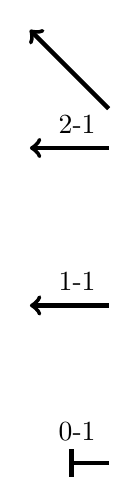
\begin{tikzpicture}
        \draw [ultra thick, <-] (0,5.5) -- (1,4.5);
        \draw [ultra thick, <-] (0,4) -- (1,4);
        \node at (0.6,4.3) {2-1};
        \draw [ultra thick, <-] (0,2) -- (1,2);
        \node at (0.6,2.3) {1-1};
        \draw [ultra thick,|-] (0.5,0) -- (1,0);
        \node at (0.6,0.4) {0-1};
    \end{tikzpicture}
    \vspace*{1em}

    \column{.45\textwidth}

    One of the best-known sauropods, Diplodocus was a very large long-necked 
    quadrupedal animal, with a long, whip-like tail.\\[1.2em]

    Its forelimbs were slightly shorter than its hind limbs, resulting in a 
    largely horizontal posture.\\[1.2em]

    It is the longest dinosaur known from a complete skeleton.

\end{columns}

\vspace*{1em}

Source~: \url{http://en.wikipedia.org/wiki/Diplodocus}

\end{frame}
%-E--------------------------------------------------------------------------E-%


%-B--------------------------------------------------------------------------B-%
\begin{frame}
\frametitle{Alignement de mots}

Exemple d'alignment simple.

\begin{center}
Je suis Français . \\
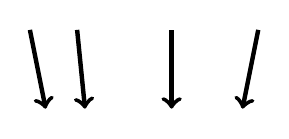
\begin{tikzpicture}
    \draw [ultra thick, <-] (0.4,0) -- (0.2,1);
    \draw [ultra thick, <-] (0.9,0) -- (0.8,1);
    \draw [ultra thick, <-] (2,0) -- (2,1);
    \draw [ultra thick, <-] (2.9,0) -- (3.1,1);
\end{tikzpicture}\\[-0.2em]
I am French .
\end{center}

\vspace*{1em}

Exemple d'alignment plus compliqué.

\begin{center}
Je m' appelle Paul . \\
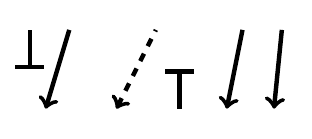
\begin{tikzpicture}
    \draw [ultra thick, |-] (0.4,0.5) -- (0.4,1);
    \draw [ultra thick, <-] (0.6,0) -- (0.9,1);
    \draw [dashed, ultra thick, <-] (1.5,0) -- (2,1);
    \draw [ultra thick, -|] (2.3,0) -- (2.3,0.5);
    \draw [ultra thick, <-] (2.9,0) -- (3.1,1);
    \draw [ultra thick, <-] (3.5,0) -- (3.6,1);
\end{tikzpicture}\\[-0.2em]
My name is Paul .
\end{center}

\end{frame}
%-E--------------------------------------------------------------------------E-%

%-B--------------------------------------------------------------------------B-%
\begin{frame}
\frametitle{Corpora parallèles disponibles}

\begin{itemize}\itemsep10pt
    \item Europarl~\cite{koehn2005europarl}
    \begin{itemize}
        \item Délibérations du Parlement européen disponibles en 21 langues et 
              alignées au niveau de la phrase.
    \end{itemize}
    \item OPUS~\cite{tiedemann2009news}
    \begin{itemize}
        \item Collection de corpora parallèles issus de sources variées~:
              EMEA (European Medicines Agency documents), KDE4 (KDE4 
              localization files), Europarl, OpenSubtitles, etc.
        \item \url{http://opus.lingfil.uu.se/}
    \end{itemize}
    \item Les livres numériques librement disponibles.
    \begin{itemize}
        \item \url{http://www.gutenberg.org/}
    \end{itemize}
    \item Wikipédia~: \alert{\fbox{plus comparable que parallèle}}
\end{itemize}

\end{frame}
%-E--------------------------------------------------------------------------E-%


%==============================================================================%
\subsection{Corpus comparable}
%==============================================================================%


%-B--------------------------------------------------------------------------B-%
\begin{frame}[allowframebreaks]
\frametitle{Corpus comparable}

\begin{itemize}\itemsep10pt
    \item Les corpora parallèles sont très couteux à produire et ils ne sont
          disponibles que dans un nombre de langues/domaines réduit.
    \item Les corpus dits \textbf{comparables} sont largement plus répandus.
    \item D'après Déjean \& Gaussier~\cite{dejean2002nouvelle}~:
    \begin{itemize}
        \item Deux corpus de deux langues $l_1$ et $l_2$ sont dits comparables 
              s'il existe une sous-partie non négligeable du vocabulaire du 
              corpus de langue $l_1$, respectivement $l_2$, dont la traduction 
              se trouve dans le corpus de langue $l_2$, respectivement $l_1$.
    \end{itemize}

    \framebreak

    \item Exemple~: un ensemble d'articles de journaux dans différentes langues,
          traitant d'une même actualité et à la même époque.
    \item Applications~:
    \begin{itemize}
        \item Extraction de phrases parallèles~\cite{smith2010extracting}
        \item Constitution de dictionnaires bilingues~\cite{rapp1999automatic}
    \end{itemize}
    \item Peu (ou pas~?) de corpora comparables disponibles.
    \begin{itemize}
        \item Wikipedia
    \end{itemize}
\end{itemize}

\end{frame}
%-E--------------------------------------------------------------------------E-%


%==============================================================================%
\subsection{La constitution de corpus}
%==============================================================================%


%-B--------------------------------------------------------------------------B-%
\begin{frame}
\frametitle{La constitution de corpus}

\begin{enumerate}\itemsep10pt

    \item Définir les caractéristiques du corpus~:
    \begin{itemize}
        \item Quels sont les phénomènes que l'on souhaite observer~?
        \item Quelle est la tâche que l'on souhaite réaliser~?
        \item Le corpus doit-il pouvoir être distribué~?
    \end{itemize} 

    \item Assembler les unités textuelles (documents, phrases, etc.)
    \begin{itemize}
        \item Est-ce que le processus peut être automatisé~?
        \begin{itemize}
            \item e.g.~moissonnage à partir du web (\textit{web scraping}).
        \end{itemize}
        \item Une sélection manuelle est-elle nécessaire (et possible)~?
        \item[$\to$] Garder en mémoire la méthodologie utilisée (e.g.~README).
    \end{itemize}

    \item[Opt.] Annotation du corpus
    \begin{itemize}
        \item Annoter les unités textuelles (e.g.~\textit{Part-Of-Speech}).
        \item Créer un référenciel pour l'évaluation (e.g.~termes-clés).
        \item[$\to$] Définir des \textit{guidelines} à joindre au corpus.
    \end{itemize}

\end{enumerate}

\end{frame}
%-E--------------------------------------------------------------------------E-%

%-B--------------------------------------------------------------------------B-%
\begin{frame}
\frametitle{Exemple 1}
\framesubtitle{Corpus pour évaluer un système d'extraction de termes-clés}

\begin{itemize} \itemsep10pt
    \item Caractéristiques du corpus
    \begin{itemize}
        \item On souhaite évaluer un système d'extraction de termes-clés et 
              pouvoir distribuer le corpus pour des raisons de comparaison.
        \item[$\to$] Choix de la nature des documents~: \alert{articles}, blogs,
                     tweets, etc.
        \item[$\to$] Langue(s) des documents~: anglais, \alert{français}, etc.
        \item[$\to$] Source(s) des documents~: lemonde.fr, \alert{wikinews}, 
                     etc.
        \item[$\to$] Nombre de documents~: 10, 20, 50, \alert{100}, 1000, etc.
    \end{itemize}

    \item Récupération des documents
    \begin{itemize}
        \item Automatiser le processus à partir d'un \textit{dump} de wikinews
        \item[$\to$] Filtrage (manuel) des documents trop courts
        \item Définir un format pour les documents (XML, HTML, txt, etc.)
    \end{itemize}

    \item Création d'un référentiel pour l'évaluation
    \begin{itemize}
        % \item Recruter des annotateurs pour extraire les termes-clés
        \item Tâche subjective $\to$ plusieurs annotations par documents
    \end{itemize}

\end{itemize}

\end{frame}
%-E--------------------------------------------------------------------------E-%

%-B--------------------------------------------------------------------------B-%
\begin{frame}
\frametitle{Exemple 2}
\framesubtitle{Corpus de phrases analysées en dépendances}

\begin{itemize} \itemsep10pt
    \item Caractéristiques du corpus
    \begin{itemize}
        \item On souhaite créer un corpus composé de phrases analysées en 
              dépendances afin d'étudier des phénomènes linguistiques
              et d'entraîner un outil d'analyse en dépendances.
        \item[$\to$] Choix de la nature des phrases~: \underline{\qquad}
        \item[$\to$] Langue(s) des phrases~: \underline{\qquad}
        \item[$\to$] Source(s) des phrases~: \underline{\qquad}
        \item[$\to$] Nombre de phrases~: \underline{\qquad}
    \end{itemize}
    \item Récupération des phrases
    \begin{itemize}
        \item[$\to$] Récupération automatisée ou manuelle~?
    \end{itemize}
    \item Annotation des phrases
    \begin{itemize}
        \item Recruter des spécialistes~? définir des \textit{guidelines}~? 
    \end{itemize}

\end{itemize}

\end{frame}
%-E--------------------------------------------------------------------------E-%


%==============================================================================%
\subsection{L'annotation de corpus}
%==============================================================================%

%-B--------------------------------------------------------------------------B-%
\begin{frame}
\frametitle{L'annotation de corpus}

\begin{itemize}
    \item Différents niveaux d'annotation
\end{itemize}

\end{frame}
%-E--------------------------------------------------------------------------E-%



%-B--------------------------------------------------------------------------B-%
\begin{frame}
\frametitle{Un point sur l'encodage}

\end{frame}
%-E--------------------------------------------------------------------------E-%


%-B--------------------------------------------------------------------------B-%
\begin{frame}
\frametitle{Un point sur les méta-données}

\end{frame}
%-E--------------------------------------------------------------------------E-%


